%-------------------------------------------------------------------------------
% BIFURCATION ANALYSIS 
%-------------------------------------------------------------------------------

\section{Bifurcation Analysis and Dynamical Systems} \label{sec:bif}

Hydrodynamic stability theory studies how a fluid flow is affected by small
disturbances of an initial state. This field of fluid dynamics involves
analytical, experimental, and more and more computational explorations. Flow
regimes can be categorized as either unstable or stable. Unstable in the sense
that even infinitesimally small variations will cause the flow to deviate from
its initial state, resulting in a different flow state or the onset of
turbulence. Conversely, disturbances do not change the initial system's state
in a stable flow.

In the context of the R4CF problem, the main objective is to investigate the
behavior of the driven cavity for different configurations in a numerical
experiment. We want to mainly understand how the flow is affected by the length
of the side walls, the boundary velocity, and the fluid's viscosity. All these
quantities are captured by the Reynolds number.

In figure \ref{fig:timestepping}, it has been identified that two asymmetric
states are possible when the Reynolds number exceeds a critical threshold, and
although the symmetric base flow remains a solution to the governing equations,
it becomes unstable. The point at which the two states emerge is called a
bifurcation point. A bifurcation is the change of a value of qualitative
character of the set of possible steady and unsteady flows in dynamical
equilibrium \citep{drazin2002}. These points are often associated with
instabilities, multiple flow patterns, or the emergence of oscillatory
behavior. We recall the original bifurcation diagram presented in figure
\ref{fig:bif_diag_chen}. To understand this diagram and to differentiate the
points where the flow states are altered, we want to introduce the mathematical
underpinnings from a dynamical system point of view. After that, the occurring
bifurcations for the 4RCF will be explained in detail.

\subsection{The Dynamical Systems Perspective}

An alternative perspective on our problem at hand is through the theory of
dynamical systems. In this framework, the state of a system is represented by a
multidimensional point denoted as $x$ within a set of all possible states,
referred to as the state space or phase space (indicated as $X$). This point
describes the system's current state and includes all the necessary dimensions
to determine its future evolution.

A time variable $t \in T$ governs the evolution of a system, where $T$ in our
case is a set of positive real numbers ($T \in \mathbb{R}^+$). The evolution
operator $\varphi_t : X \to X$ is a map that describes the system's
transformation over time. For the evolution to comply with the deterministic
nature of dynamical systems, the operator must satisfy the identity map for an
initial condition $x_0$ at time zero. The second requirement is referred to as
time invariance and signifies that for any $x \in X$, the evolution operator
$\varphi_t$ remains constant over time, that is, $\varphi_t(x) = \varphi_s(x)$
for all $t, s \in T$. Now, a dynamical system can be defined with a triple $\{
T, X, \varphi^t \}$ and the above-mentioned conditions for the evolution
operator \citep{kuznetsov2004}.

The equation for the streamfunction \eqref{eq:str} is an autonomous
differential equation, which can be reformulated as a dynamical system. We
consider an infinite-dimensional point denoted as $\Psi$ in a state space $X$.
$\Psi$ can be thought of as a vector covering all possible points of our cavity
and thus is infinite-dimensional. Using the streamfunction at time $t$, we have
not only the locations of all fluid particles but also their evolution
(velocities $u$ and $v$) explicitly given by the definition of the derivatives
\eqref{eq:str_defx} and \eqref{eq:str_defy}.

Further, this infinite-dimensional space will be divided into discrete points
with the chosen pseudo-spectral discretization. Increasing $m$ should result in
higher accuracy, and the solution is expected to converge exponentially because
of the singularity-avoiding regularization. The finite-dimensional space for
the numerical computations can be defined as:
\begin{align}
  \frac{d(\Delta \Psi_j)}{dt} &= {F_j(\Psi)} \quad \quad \quad
    j= 1,2,\dots,(m+1)(n+1), \label{eq:dyn_sys}
\end{align}

where $F_j$ to the $j$th component of the nonlinear function for one grid
point. Equations \eqref{eq:dyn_sys} is essentially a dynamical system of
$(m+1)(n+1)$ equations.

This more abstract framework is helpful in the sense that it provides a
geometrical representation of the sought-after solutions. It is of use to look
at subsets of the phase space $X$. A first example is an invariant set which is
a subset $S$ such that an $x_0$ implies $\varphi(x_0) \in S$ for all $t \in T$
\citep{kuznetsov2004}. If $S$ is just one single point (having measure $0$)
this set is called a fixed point (or equilibrium). 

Additionally, an invariant manifold corresponds to a hypersurface such that all
future time maps of the evolution operator reside on this surface. Trajectories
on such manifolds are termed periodic orbits and are trajectories in phase
space that will revisit the same state again. \red{A limit cycle or stable
periodic orbit is a trajectory that will be visited repeatedly. Such limit
cycles are defined by being isolated and attracting, attracting other close-by
trajectories}. Further, periodic orbits can be classified by their period and
amplitude and are usually depicted in what is called a phase portrait. These
invariant sets help to characterize dynamical systems and understand the
fundamental types of solutions when a parameter of interest is varied.

\subsection{Steady-State Solutions}

We have seen that launching a time stepper gives different kinds of states
depending on the initial condition. A steady-state solution corresponds to the
solution of the differential equation where the time $t$ approaches infinity.
Moreover, this is exactly a fixed point (and invariant set) that can be
obtained by setting the time-dependent term to zero. All of our steady-state
solutions satisfy the following equation:
\begin{align}
  F(\Psi, \Rey) & = \frac{1}{\Rey}\Delta^2 \Psi +
    (\partial_x \Psi) \partial_y(\Delta \Psi) -
    (\partial_y \Psi) \partial_x(\Delta \Psi) \nonumber \\
  & =  0 \label{eq:str_steady}
\end{align}

As the outer two grid rows and columns are explicitly known through the
boundary conditions (explained in section \ref{sec:bc}), a reduced system of
equations, $F(\psi, \Rey) = 0$, can be formulated. $\psi \in
\mathbb{R}^{(m-1)\times(n-1)} $ corresponds now to the inner grid points. 

Practically in the case of the two-dimensional cavity flow, we will have system
of $(m-3)(n-3)$ equations and can solve this equation analogously to the
time-stepping equation with a Newton iteration.

\subsection{Linear Stability Analysis}

To analyze the stability of fixed points, a mathematical technique called
linear stability analysis can be used. Given an equilibrium solution $\Psi_0$,
which is a solution to the steady equation \eqref{eq:str_steady}, we can try to
perturb the system and see how it would behave. Let us define a perturbated
$\Psi$,
\begin{align}
\Psi = \Psi_0 + \epsilon \tilde{\Psi},
\end{align}

where $\epsilon$ is a small disturbance. We can insert this expression into the
time-dependent streamfunction equation. By only looking at first-order terms
$\mathcal{O}(\epsilon)$ and using the fact that $F_{steady}(\Psi_0) = 0$, we
get
\begin{align}
\partial_t \Delta \tilde{\Psi} = \frac{1}{Re} \Delta^2 \tilde{\Psi}
  + (\partial_x \Psi_0) \partial_y (\Delta \tilde{\Psi})
  + (\partial_x \tilde{\Psi}) \partial_y (\Delta \Psi_0)
  - (\partial_y \Psi_0) \partial_x (\Delta \tilde{\Psi})
  - (\partial_y \tilde{\Psi}) \partial_x (\Delta \Psi_0)
\label{eq:str_pert}
\end{align}

To solve this linear stability analysis problem, an Ansatz is used, where we
separate time and the spatial variables as follows: 
\begin{align}
  \tilde{\Psi} = \tilde{\Psi}(x,y,t) = \mathrm{e}^{\lambda t} \Phi(x,y)
\end{align}

$\Phi$ only corresponds to a component of the solution that depends only on $x$
and $y$. The time variable $t$ can then be eliminated by plugin the above back
into the equation.
\begin{align}
\lambda \Delta \Phi = \frac{1}{Re} \Delta^2 \Phi
  + (\partial_x \Psi_0) \partial_y (\Delta \Phi)
  + (\partial_x \Phi) \partial_y (\Delta \Psi_0)
  - (\partial_y \Psi_0) \partial_x (\Delta \Phi)
  - (\partial_y \Phi) \partial_x (\Delta \Psi_0)
\label{eq:str_phi}
\end{align}

This resulting equation is a generalized eigenvalue problem. In terms of two
operators $A$ and $B$, the problem can be stated as follows: 
\begin{align} \label{eq:eig_prob}
  \begin{split}
  A \Phi & = \lambda B \Phi \\[4pt]
  \begin{split}
  A & = \frac{1}{Re} \Delta^2 \bullet
    + (\partial_x \Psi_0) \partial_y (\Delta \bullet)
    + (\partial_x \bullet) \partial_y (\Delta \Psi_0) \\
    &\quad - (\partial_y \Psi_0) \partial_x (\Delta \bullet)
    - (\partial_y \Phi) \partial_x (\Delta \Psi_0)
  \end{split} \\
  B & = \Delta
  \end{split}
\end{align}

We recognize that $\Phi(x,y)$ corresponds to an eigenmode, and $\lambda$ is the
associated eigenvalue. If all the eigenvalues of the generalized eigenvalue
problem have a positive real part, the equilibrium is stable. On the contrary,
if only one of the eigenvalues is found to be positive, then the system is
unstable because a small perturbation will grow exponentially in time, which
can be directly seen in the definition of the Ansatz.

This linear stability problem becomes computationally demanding because the
perturbation $\epsilon$ has to be performed on every grid point, and the
numerical eigenvalue problem is solved with matrices of the size $(m+1)(n+1)
\times (m+1)(n+1)$. A final remark is that with linear stability analysis, we
are only looking at linear perturbation, meaning that nonlinear disturbances
(second or higher order) are not captured with this technique.

\subsection{Bifurcations} \label{sec:bif_details}

We have formally defined the tools needed to characterize all the bifurcations
occurring in the RCF4 precisely. 

To illustrate the bifurcations we encountered, a parameter of interest $\mu$
($\Rey$ in the RC4F) will be varied and plotted against a variable that
identifies a different state. Let denote this variable by $U$ ($\Psi_{center}$
in the RCF4). The first bifurcation we want to look at is the pitchfork (figure
\ref{fig:pitch_saddle}), where the symmetry of a problem is broken, and two
different flow solutions appear. The base solution is still in equilibrium but
now unstable.

\begin{figure}[ht]
\centering
\begin{subfigure}[t]{0.3\textwidth}
  \centering
  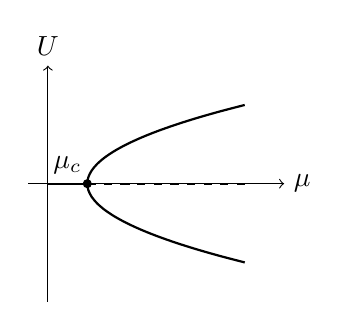
\begin{tikzpicture}[scale=0.5]
    \draw[->] (-0.5,0) -- (6,0) node[right] {$\mu$};
    \draw[->] (0,-3) -- (0,3) node[above] {$U$};
    
    \draw[thick] plot[smooth,domain=-2:2] ({1 + \x*\x},\x);
    \draw[thick] plot[smooth,domain=0:1] (\x,0);
    \draw[thick] plot[smooth,domain=0:1] (\x,0);

    \draw[thick, dashed] plot[smooth,domain=1:5.2] (\x,0);
    \draw[thick, dashed] plot[smooth,domain=1:5.2] (\x,0);
    
    \draw[fill=black] (1,0) circle (0.1);
    \node[above left] at (1.1,0) {$\mu_c$};
  \end{tikzpicture}
\end{subfigure}
\hspace{0.1\textwidth}
\begin{subfigure}[t]{0.3\textwidth}
  \centering
  \begin{tikzpicture}[scale=0.5]

  \draw[->] (-0.5,0) -- (6,0) node[right] {$\mu$};
  \draw[->] (0,-3) -- (0,3) node[above] {$U$};

  \draw[thick, dashed] plot[smooth,domain=-1.9:0] ({5 - 1.2*\x*\x},\x);
  \draw[thick] plot[smooth,domain=0:1.9] ({5 - 1.2*\x*\x},\x);

  \draw[fill=black] (5,0) circle (0.1);
  \node[above right] at (5,0) {$\mu_c$};
  \end{tikzpicture}
\end{subfigure}
\caption{Supercritical pitchfork bifurcation (left) and a saddle-node (right)}
  \label{fig:pitch_saddle}
\end{figure}

Another type of bifurcation is called a saddle-node or fold bifurcation, where
a set of stable and unstable fixed points collide. In a bifurcation diagram in
(figure \ref{fig:pitch_saddle}), this is characterized by a saddle point hence
the name.

Lastly, a Hopf is a bifurcation where a stable fixed point loses its stability,
and from the critical parameter value onwards, we have unstable or stable
periodic orbits. This is characterized by a real complex conjugate pair of
eigenvalues crossing when performing the stability analysis. One can
distinguish between sub- and supercritical Hopf bifurcation. At a Hopf
bifurcation, a stable fixed point becomes unstable, and the system suddenly
oscillates. A sketch of the amplitudes is depicted in figure \ref{fig:hopf}.
Compared to local bifurcation, such as pitchfork and saddle-node, this is
called a global bifurcation. The global behavior is seen, for example, in the
supercritical Hopf when the system is changing suddenly from a fixed point to a
stable periodic orbit (SPO) and now following a trajectory in a larger
invariant set when we think in terms of dynamical systems. On the other hand,
the subcritical Hopf is less predictable. Before the critical $\mu$, there are
unstable periodic orbits, and then it is unclear what the amplitudes of
oscillations will be when the fixed point becomes unstable.

\begin{figure}[ht]
\centering
\begin{subfigure}[t]{0.3\textwidth}
  \centering
  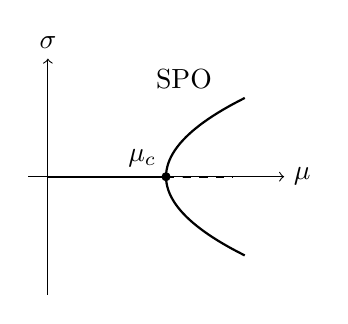
\begin{tikzpicture}[scale=0.5]
    \draw[->] (-0.5,0) -- (6,0) node[right] {$\mu$};
    \draw[->] (0,-3) -- (0,3) node[above] {$\sigma$};
    
    \draw[thick] plot[smooth,domain=-2:2] ({3 + 0.5*\x*\x},\x);
    \draw[thick] plot[smooth,domain=0:3] (\x,0);
    \draw[thick] plot[smooth,domain=0:3] (\x,0);

    \draw[thick, dashed] plot[smooth,domain=3:4.7] (\x,0);
    \draw[thick, dashed] plot[smooth,domain=3:4.7] (\x,0);
    
    \draw[fill=black] (3,0) circle (0.1);
    \node[above left] at (3,0) {$\mu_c$};

    \node[above right] at (2.5,2) {SPO};
  \end{tikzpicture}
\end{subfigure}
\hspace{0.1\textwidth}
\begin{subfigure}[t]{0.3\textwidth}
  \centering
  \begin{tikzpicture}[scale=0.5]
    \draw[->] (-0.5,0) -- (6,0) node[right] {$\mu$};
    \draw[->] (0,-3) -- (0,3) node[above] {$\sigma$};
    
    \draw[thick, dashed] plot[smooth,domain=-2:2] ({3 - 0.5*\x*\x},\x);
    \draw[thick] plot[smooth,domain=0:3] (\x,0);
    \draw[thick] plot[smooth,domain=0:3] (\x,0);

    \draw[thick, dashed] plot[smooth,domain=3:4.7] (\x,0);
    \draw[thick, dashed] plot[smooth,domain=3:4.7] (\x,0);
    
    \draw[fill=black] (3,0) circle (0.1);
    \node[above right] at (3,0) {$\mu_c$};

    \node[above right] at (1.5,2) {PO};
  \end{tikzpicture}
\end{subfigure}
\caption{Sketch of amplitudes of stable (SOP) and unstable (PO) periodic orbits for supercritical (left) and subcrititical Hopf (right), }
\label{fig:hopf}
\end{figure}

\subsection{Continuation Algorithms} \label{sec:cont}

The next key idea is how to track branches of fixed points. The simplest
numerical algorithm is called natural continuation, where we start with a
solution obtained by a time-stepper and then increase the Reynolds number. The
initial guess for the next Newton iteration is the solution of the step before.
In this way, we can "continue" a branch without using a time integration
algorithm for each steady-state solution we want to obtain. The Newton method
will converge if the steps in $\mu$ are small enough. Furthermore, unstable
branches can be followed as well, which can not be done solely by time
evolution.

However, there is a limitation. In the fold bifurcation depicted in figure
\ref{fig:pitch_saddle}, the continuation has to follow a curve when the
parameter is decreasing again. The natural continuation cannot properly achieve
this, as the Reynolds number is manually set to increase. Another strategy to
overcome this issue is called pseudo-arclength continuation
\citep{kuznetsov2004}. Given two fixed points $x^{(0)}$ and $x^{(1)}$ on a
curve with parameter values $\mu^{(0)}$ and $\mu^{(1)}$ we want to find the
next $x^{(2)}$ and $\mu^{(2)}$ making a prediction with the approximated
tangents from the already given fixed points:
\begin{equation}
  \tilde{x}^{(2)} = x^{(1)}  + \underbrace{[x^{(1)} - x^{(0)}]}_{\text{\normalfont $\hat{x}$}} \gamma
\end{equation}

Here $\gamma$ (in this study set to $1$) is a parameter that determines the
prediction step size. $\tilde{x}^{(2)}$ is called the predictor. Now we want to
impose another equation with what is called the correction step.
\begin{equation}
  (x^{(2)} - x^{(1)})  \cdot \hat{x} \label{eq:extra}
\end{equation}

This equation tells us that we want to find the next point on the curve that is
orthogonal in our phase space to the tangent drawn from our previous points.
Figure \ref{fig:pseudo_cont} illustrates this idea geometrically.

Consequently, $\mu^{(2)}$ is determined explicitly by satisfying the equation
\eqref{eq:extra}. To find the next point, the initial system of nonlinear
equations \eqref{eq:dyn_sys} is augmented by:
\begin{equation}
  F(x^{(2)}, \mu^{(0)}) = 
\begin{bmatrix} F(x^{(2)}, \mu) \\ (x^{(2)} - x^{(1)})  \cdot \hat{x},
\end{bmatrix} \label{eq:dyn_sys_cont}
\end{equation}

and this means the parameter $\mu$ is now part of the equation. The augmented
Jacobian can be formulated as follows: 
\begin{equation}
\renewcommand\arraystretch{1.5}
J = 
\left[
\begin{array}{cc}
  J_x \quad \quad \quad \quad & F_{\mu} \\
  \hdashline
  \quad (x^{(2)} - x^{(1)})^T
\end{array} \label{eq:jac_aug}
\right]
\end{equation}

So we, first of all, calculate the original Jacobian $J_x$, and the components
of the last row of the augmented Jacobian are given by the transpose of the
distance in phase space, between the two already computed states. The last
column (without the last row) corresponds to the finite difference derivative
of the nonlinear function with respect to $\mu$. It is necessary to scale the
parameter $\mu$ to obtain changes with similar magnitudes as for the $x$
components. This ensures a well-conditioned Jacobian.

\begin{figure}[h]
\centering
\begin{tikzpicture}
  \draw[->] (0,-0.5) -- (0,4) node[above] {$"x"$};
  \draw[->] (-0.5,0) -- (4,0) node[right] {$\mu$};

  \draw[smooth, thick, variable=\x, domain=0.5:4] plot ({\x},{2 - 0.25*(\x - 2.5)^2});

  \draw[fill=black] (0.6,{2 - 0.25*(0.6 - 2.5)^2}) circle (0.05) node[below] {$x^{(0)}$};
  \draw[fill=black] (1.2,{2 - 0.25*(1.2 - 2.5)^2}) circle (0.05) node[below] {$x^{(1)}$};

  \draw[dashed] (0.6,{2 - 0.25*(0.6 - 2.5)^2}) -- (2.5,{0.6 + ((2 - 0.25*(1.2 - 2.5)^2) - (2 - 0.25*(0.6 - 2.5)^2))/0.6*2.5});

  \draw[dashed] ((2.5,{0.6 + ((2 - 0.25*(1.2 - 2.5)^2) - (2 - 0.25*(0.6 - 2.5)^2))/0.6*2.5}) -- (3,{2 - 0.25*(3 - 2.5)^2});

  \draw[fill=black] ((2.5,{0.6 + ((2 - 0.25*(1.2 - 2.5)^2) - (2 - 0.25*(0.6 - 2.5)^2))/0.6*2.5}) 
    circle (0.05) node[above] {$\tilde{x}^{(2)}$};;
  \draw[fill=black] (3,{2 - 0.25*(3 - 2.5)^2}) circle (0.05) node[below] {$x^{(2)}$};;
\end{tikzpicture}
\caption{Pseudo-arclength continuation, a simplified illustration by projecting the vector $x$ on a plane}
\label{fig:pseudo_cont}
\end{figure}
